% Figure 3 of docs/exposition.md: comparisons on the cycled board of
% Section 4. An arrow i -> j means that column i beats column j (a_ij = 1 with
% exact decoding). Build with tools/render_papers.py.
\documentclass[tikz,border=4pt]{standalone}
% Shared TikZ style for the figures of docs/exposition.md.
% Palette and bit cells follow docs/figures/expert_column.tex.
\usepackage{amsmath,amssymb}
\usetikzlibrary{arrows.meta,positioning,calc,decorations.pathreplacing}
\definecolor{one}{RGB}{226,232,240}
\definecolor{zero}{RGB}{40,40,40}
\definecolor{win}{RGB}{176,58,46}
\definecolor{addr}{RGB}{40,90,150}
\definecolor{lose}{RGB}{110,110,110}
\tikzset{
  bit/.style={draw=black!60, minimum width=4.4mm, minimum height=4.4mm,
              inner sep=0pt, font=\scriptsize},
  onebit/.style={bit, fill=one},
  zerobit/.style={bit, fill=zero, text=white},
  cell/.style={draw=black!50, fill=white, minimum width=10mm,
               minimum height=4.2mm, inner sep=0pt, font=\scriptsize},
  >={Stealth[length=2.2mm]}}

% \boardcolumn{name}{x}{b1}{b2}{b3}{b4}{address text}
% Draws X_name as four bits at height 0 starting at x, the address inputs
% below, and the four cells 00,01,10,11 named <name>c00 ... <name>c11.
\newcommand{\boardcolumn}[7]{%
  \node[anchor=east, font=\small] at (#2-0.05,0) {$X_{#1}$};
  \foreach \c/\b in {1/#3,2/#4,3/#5,4/#6} {
    \ifnum\b=0
      \node[zerobit] (x#1-\c) at (#2+0.46*\c-0.23,0) {0};
    \else
      \node[onebit] (x#1-\c) at (#2+0.46*\c-0.23,0) {1};
    \fi}
  \node[font=\scriptsize, align=center, addr, anchor=north] (adr#1)
    at (#2+0.92,-0.38) {#7};
  \foreach \s/\k in {00/0,01/1,10/2,11/3} {
    \node[cell] (#1c\s) at (#2+0.92,-1.62-0.5*\k) {$B_{#1,\s}$};}
}

\begin{document}
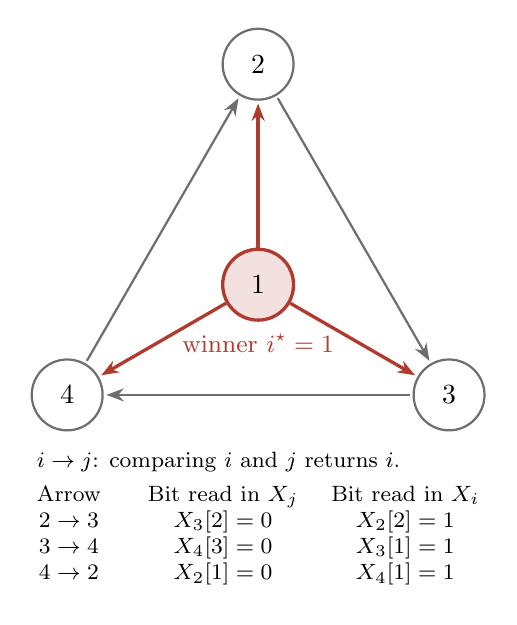
\begin{tikzpicture}[
  col/.style={circle, draw=lose, thick, minimum size=9mm, font=\normalsize, fill=white},
  beat/.style={->, thick, lose, shorten >=1pt, shorten <=1pt}]
\node[col, draw=win, fill=win!15, very thick] (c1) at (0,0) {$1$};
\node[col] (c2) at (90:2.8) {$2$};
\node[col] (c3) at (-30:2.8) {$3$};
\node[col] (c4) at (210:2.8) {$4$};
\node[win, font=\small, align=center, anchor=north] at (0,-0.5)
  {winner $i^\star=1$};
\foreach \j in {2,3,4} \draw[->, win, very thick, shorten >=1pt] (c1) -- (c\j);
\draw[beat] (c2) -- (c3);
\draw[beat] (c3) -- (c4);
\draw[beat] (c4) -- (c2);
\node[font=\footnotesize, align=left, anchor=north] at (0,-2.0)
  {$i\to j$: comparing $i$ and $j$ returns $i$.\\[3pt]
   \begin{tabular}{@{}c@{\qquad}cc@{}}
     Arrow & Bit read in $X_j$ & Bit read in $X_i$ \\
     $2\to3$ & $X_3[2]=0$ & $X_2[2]=1$ \\
     $3\to4$ & $X_4[3]=0$ & $X_3[1]=1$ \\
     $4\to2$ & $X_2[1]=0$ & $X_4[1]=1$
   \end{tabular}};
\end{tikzpicture}
\end{document}
